\chapter{\minstrel/ and \skald/}

\label{ch:skald}

\skald/ is an open-source\footnote{\skald/'s source code is available at \url{https://sites.google.com/a/soe.ucsc.edu/eis-skald/}} narrative generator that was created via a process of rational reconstruction, using Scott Turner's 1993 \minstrel/ as the object of study.
%
Like \minstrel/, it has an underlying graph-based representation of stories, and constructs new graphs via a case-based reasoning process that draws on a fixed library of pre-authored story graphs.
%
I worked on \skald/ with Brandon Tearse, and together we re-created \minstrel/'s original functionality and then used \skald/ to study \minstrel/'s strengths and weaknesses \citep{Tearse2011, Tearse2012, Tearse2014}.
%
This section explains how \skald/ works, and then discusses what we learned from building it, and ultimately, why I was unsatisfied with Turner's imaginative recall process for constructing stories.



\section{Rational Reconstruction}


Before getting in to the details of \skald/, a brief note about rational reconstruction, which was our methodology for constructing \skald/ based on \minstrel/.
%
As a technical approach in computer science, rational reconstruction begins with in-depth study of an existing system, so that it can be understood at an algorithmic level (see e.g., \citep{Peinado2006}, which is closely related to \skald/, or \citep{Musen1995}).
%
If the system is available for direct study, this includes inspecting the source code and running the original system to see how it behaves.
%
If not, descriptions of the original system's behavior are used to understand how it functions.


Once a system's behavior is well-understood, rational reconstruction proceeds by developing a new codebase to reproduce the functionality of the original.
%
The reason not to use the original code is that developing new code is a means of exposing quirks in the original.
%
Large software projects often contain implicit architectural decisions that are the result of idiosyncrasies in the original code.
%
The original programmer(s) may have been unaware of these decisions, as in their implementation the programming language, or some other feature of their code design, precluded some alternatives.
%
By developing a separate codebase, often in a different programming language from the original, rational reconstruction projects can expose these implicit properties of the original software, and thus learn more about the algorithm being investigated.
%
Rational reconstruction as a technical approach thus echoes rational reconstruction as a philosophical or historical approach in that it works ``from the outside'' and seeks formal systems of representation that differ from those of its subject as a means of creating a productive alternative perspective (see e.g. \citep{Lakatos1971} for several examples of how rational reconstruction has been applied to the history of science).


For our work on \skald/, we got in touch with Turner, who graciously offered to supply us with magnetic tapes containing \minstrel/'s source code.
%
Given that we had neither a magnetic tape reader nor a machine that could run \minstrel/'s LISP variant on hand, we decided to proceed without the source code, using Turner's dissertation as the reference for \minstrel/'s design.
%
Turner's dissertation includes detailed descriptions of all of \minstrel/'s
modules, in addition to several appendices, one of which contains an annotated
trace of a run of \minstrel/.



\section{\skald/}


Turner called \minstrel/'s core operating principle ``imaginative recall.''
%
Humans often make up new stories using pieces of stories they've heard in the past, and Turner reasoned that a computer could operate using the same principle: supplied with a story library, it could recall fragments from that library and modify them to fit together into a new story.
%
Turner was interested in computational creativity, and set out to demonstrate that a computer program could exhibit some of the same kinds of creativity as humans do when making up stories.


Besides imaginative recall, Turner's \minstrel/ used a system of what he called ``author-level plans'' (ALPs) to guide the story generation process.
%
Each ALP took a partially-finished story and helped move it towards completion in some way, usually making use of imaginative recall to fill in some part of the story.
%
Turner's ALPs were responsible for some of the higher-level story structures that \minstrel/ could generate, but \minstrel/ also started each story from a template which dictated a general moral or lesson that the story would convey.

\section{Story Templates and the Story Library}

As a case-based reasoning system, \minstrel/ relies heavily on its story library.
%
Furthermore, \minstrel/ starts each new story by importing a story template from its template library, which is another source of human-authored content.
%
In \minstrel/ and \skald/, both of these resources are represented in a unique graph-based format which \minstrel/ uses to represent all story content.


\begin{figure}[!p]
  \centering
  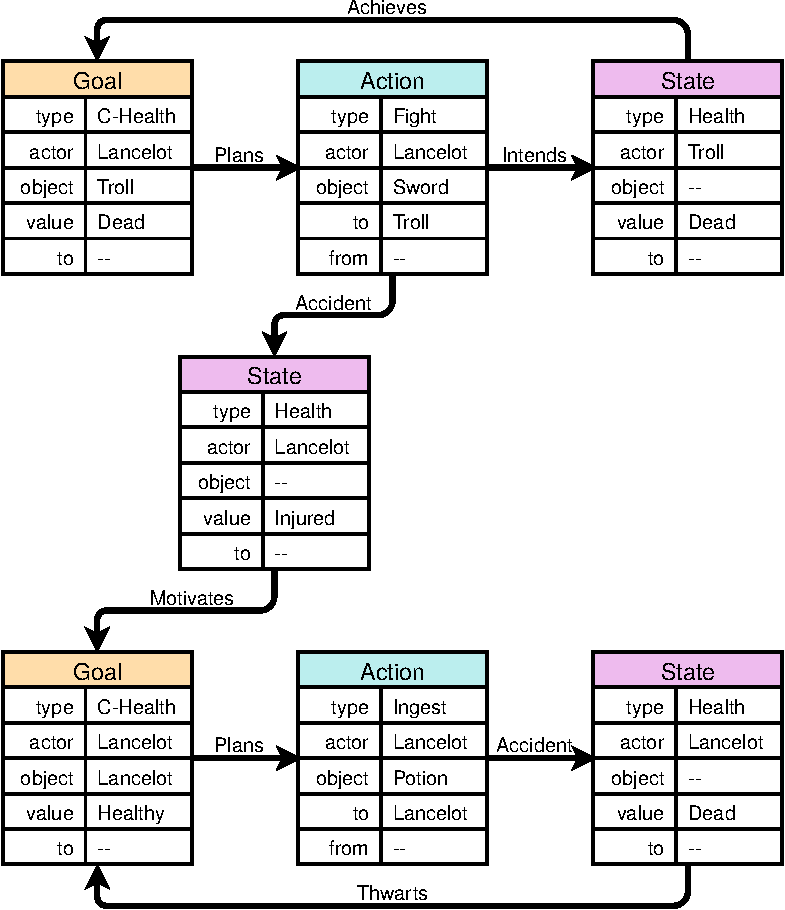
\includegraphics[width=\textwidth]{fig/cropped-story-graph.pdf}
  \caption[Example Skald story graph]{An example of a \skald/ story graph. It represents a story where Lancelot plans to kill a troll, attacks it with his sword and kills it, but becomes injured. After that, Lancelot wants to heal himself so he drinks a potion, but the potion kills him instead.}
\label{fig:story-graph}
\end{figure}


\minstrel/'s story graphs are directed graphs where each node is a conceptual dependency schema and edges are relations between these.
%
The four core node types are \gng/, \gna/, \gns/, and \gnb/ nodes, and they are usually found in \gng/-\gna/-\gns/ triangles linked by \gep/, \gei/, and \gea/ links.
%
Essentially, these \gng/-\gna/-\gns/ triples each represent a single event (along it its motivation and outcome) and they are linked to each other when the \gns/ of one triple has a \gem/ link to the \gng/ of another.
%
Within each node, the details of a particular \gng/, \gna/, \gns/, or \gnb/ are represented using conceptual dependency schemas, as shown in \cref{fig:story-graph}.


A few of the stories from \minstrel/'s original library are described in Turner's dissertation, but Turner's complete library was not available to us.
%
Because of this, we created our own ad-hoc story library by hand-authoring several stories that we thought would provide interesting source material.
%
One of the things we learned from this was that \minstrel/'s story library must be carefully managed to avoid generating malformed stories (this point is discussed in more detail in both \citep{Tearse2012} and \citep{Tearse2014}).
%
In particular, whenever there are multiple ways to represent the same concept in terms of story graph nodes, if different stories in the library use different encodings, the results of the imaginative recall process may be poor.
%
The same was true of \minstrel/'s starting templates: the templates had to match the story library closely in order to generate sensible stories.


\section{Author-Level Plans}

\minstrel/'s author-level plans are essentially black-box code fragments that modify a story during construction.
%
Each plan is invoked in response to an author-level goal (ALG) and can itself add new ALGs to the current generation process.
%
There can be multiple plans which can satisfy a single goal, in which case they are tried in a fixed order until one is found whose preconditions are met.
%
ALGs are stored in a priority queue, and if a selected plan fails to achieve the current goal, that goal is re-enqueued at a lower priority level (until it falls below a priority threshold at which it is marked as permanently failed).


This system allows the results of one plan to inform the operations of another when they both consider overlapping regions of the growing story graph.
%
Once all goals have been achieved, the story is considered finished.
%
The first goal of the system (called simply ``tell story'') is invoked after a story template has been imported, and it assigns both an ``instantiate'' and a ``check consistency'' goal to each node in the imported template.
%
The plans invoked to achieve these goals are responsible for most of the generated story, although there are a few plans which run under certain conditions that add additional nodes to the imported template as opposed to simply filling in empty schema fields.


One category of these template-expanding plans is the ``make-consistent'' plans.
%
These are triggered by consistency goals that arise when consistency-checking plans (triggered by the ``check consistency'' goals added by ``tell story'') find an inconsistent node.
%
For example, the \texttt{Check\abr/Goal\abr/Consistency} plan (which satisfied the ``check consistency'' goal for \gng/ nodes) might find a goal which is lacking a motivating state.
%
In this case, it could trigger the \texttt{Make\abr/Consistent\abr/Motivating\abr/State} plan, which adds a new \gns/ node linked to the \gng/ node by a \gem/ edge and adds a new ``instantiate'' ALG targeting the added node.
%
In this manner, the original story graph can be expanded during generation; \minstrel/ is not simply a complicated mad-libs system.


Although \minstrel/ and \skald/ both contain more than 20 ALPs, the single ALP that is responsible for most of the story content generated is the \texttt{General\abr/Instantiate} plan.
%
This plan is quite simple at the code level: it looks at the node in consideration along with its neighbors in the story graph, and asks the imaginative recall system to fill in the node based on the story library.
%
Of course, the operation of the imaginative recall system (\minstrel/'s case-based reasoning engine) is quite complex, and it is mostly responsible for the creative aspects of \minstrel/'s stories.


\section{Imaginative Recall}

Turner's goal in developing \minstrel/ was to demonstrate the creative potential of imaginative recall, and in particular, how it could recreate elements of of human narrative creativity.
%
Working with stories represented in terms of graphs of story schemas as described above, imaginative recall makes new stories using a story library by taking an incomplete story fragment and filling it in using a similar scene from the story library.
%
For example, a scene where a knight slays a dragon might be recalled when building a story in which a troll is killed, filling in a knight as the protagonist in the new story.
%
Intuitively, imaginative recall recognizes trolls and dragons are similar because they are both monsters, and so the scene where the knight slays the dragon is appropriate source material for the new story.


\begin{figure}[!t]
\centering
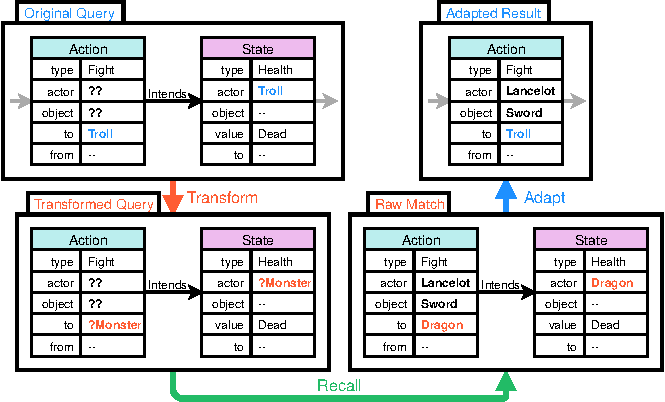
\includegraphics[width=\textwidth]{fig/cropped-im-example.pdf}
\caption[Imaginative recall example]{An example of imaginative recall using a Transform Recall Adapt method (TRAM). The original query (top left) must be Transformed (bottom left) before a match can be Recalled from the story library (bottom right). The match is then Adapted to fill in the query's target node (context nodes are discarded). Note that each empty slot is potentially connected with others in the graph, so that when ``Lancelot'' is chosen as the actor here other slots corresponding to that same actor will also be changed to ``Lancelot.''}
\label{fig:im-example}
\end{figure}


Imaginative recall actually works via a three-step recursive process: Transform, recall, and adapt.
%
First, an input query is transformed so that it can more easily match story fragments from the story library.
%
Second, a matching fragment is picked out from the library.
%
Finally, the matching fragment is adapted so that it matches the context of the current story.
%
In \cref{fig:im-example}, the query is a scene in which a troll is killed.
%
This is represented as an \gna/ node liked to a \gns/ node with an \gei/ link.
%
The \gna/ node specifies that the type of action is ``fight,'' and that a troll is the target, but the actor and tool in this case are still unknown (otherwise the story fragment would already be complete).
%
The \gns/ node specifies that the troll has a health value of ``dead,'' and it doesn't have any unknowns.


Using this query, the imaginative recall system begins by searching for a direct match in the story library: a graph fragment in which all of the fields match with the query (for unknown fields of the query, any value can match).
%
Usually, there is no exact match, as would be the case here if the story library didn't contain any stories about trolls.
%
At this point, the system would begin to consult its library of Transform Recall Adapt Methods (or TRAMs).
%
Each TRAM specifies a specific transformation of a query, along with the steps needed to undo that transformation during the adapt step.
%
Various TRAM selection strategies are possible, including anything from random selection to exhaustive search through the space of possible TRAM applications.
%
Because multiple TRAMs can be applied to a single query, there's effectively a search space of TRAM applications branching out from each starting query, and somewhere within that space (hopefully) is a query that has an exact match with a fragment in the story library.
%
Ultimately, the odds of a match increase as more TRAMs are applied, because each TRAM tends to generalize the query.


Coming back to our example, in the case of the troll being slain by an unknown actor, one available transformation is the ``GeneralizeActor'' transformation.
%
This TRAM says that a specific actor, like ``a troll,'' can be replaced with a generic actor of the specific actor's type (using a simple type ontology of actors).
%
In this case, the TRAM replaces all occurrences of the troll in the query fragment with ``a generic monster.''
%
After transformation, the new query is checked against the story library, and this time, there's a result: the scene where Lancelot the knight kills a dragon now matches our fragment, because the dragon can match ``a generic monster.''
%
Having Recalled a scene from the story library, the Adapt step is triggered.
%
In this case, the adapt part of the ``GeneralizeActor'' TRAM indicates that the actor which matched the generalized actor from the story library scene should be replaced by the actor that was generalized.
%
So the fragment from the library in which a knight slays a dragon is adapted by replacing the dragon with our specific troll.
%
If multiple TRAMs had been necessary to find a match, their adapt steps would all have been applied in reverse order.
%
The adapted story fragment can be incorporated into the story, in this case our result is that a knight kills the troll with his sword (see \cref{fig:im-example}).
%
The TRAM process has eliminated all of our initial unknowns, and this story fragment is now completed; the ALP system takes over again to select a new place fragment for imaginative recall.

\section{\minstrel/'s Potential}

The promise of imaginative recall and the TRAM system is that TRAMs can capture how story scenes can be similar to one another, and then any corpus that can be turned into a story library can become a source for generating new material.
%
Turner acknowledged that some content-specific TRAMs might be needed, and some specific to his Arthurian domain were included in \minstrel/, but these were a minority.
%
And Turner demonstrated that the TRAM system could create stories that the system had never seen before: it didn't just regurgitate what was in the story library.
%
For example, \minstrel/ was able to ``invent'' the concept of suicide by taking a scene where someone was killed and ultimately filling in the killer and the victim with the same person.
%
Because of the kinds of information embedded in \minstrel/'s story graphs, this process isn't just chaos either: \gng/ and motivating \gns/ nodes constrain how their neighboring \gna/ nodes are filled in and enforce some semblance of believability.


However, despite the potential of \minstrel/'s imaginative recall process, it is fundamentally not robust.
%
When building \skald/ we imagined that after providing a new story library containing roughly a dozen stories and doing some minor tuning, we'd be able to have \skald/ generate dozens to hundreds of new stories that included significant variations.
%
Unfortunately, what we found was that the authoring of the story library, the story templates, as well as the particular TRAMs and ALPs all had to be carefully balanced against each other to avoid nonsensical results.


In our early evaluations of the TRAM system (see \citep{Tearse2011}), we found that generating 1000 results for a single TRAM query using our new library resulted in an average of only 35.2\% sensible results: the remaining 64.8\% of results were somehow nonsensical (note that these numbers included duplicate results).
%
We tested several alternate configurations, and found that by removing some TRAMs which generalized queries too strongly, we could increase the sense-to-nonsense ratio and get an average of 92.4\% sensible results (again including duplicates).
%
Unfortunately, the removal of these TRAMs reduced the number of unique results per 1000 queries from an average of 69.4 to an average of 12, and it accordingly reduced the average number of significant differences expected between any two results from  6.9 to 3.1 (where a significant difference is something like substitution of one character for another; see \citep{Tearse2011} for methodological details).
%
This result was early evidence of the shape of the tradeoff between sense and variety in results, but it only involved the TRAM system.


Once the full reconstruction of \minstrel/ was complete, including the ALP system, we took some more measurements of TRAM query results in the context of generating full stories (see \citep{Tearse2012}).
%
We compared a vanilla version of \skald/ with a version that used modified boredom and TRAM selection systems in an attempt to trade off some variety for more consistency.
%
The modified version was able to resolve TRAM queries using much less effort (72.2\% vs. 59\% direct matches; 7.7 vs. 13.8 average TRAMs tried per successful query) largely due to the relaxed boredom restrictions.
%
However, the average number of TRAMs used in each non-direct match fell from 2.38 in the vanilla configuration to 1.39 in the modified version: in other words, the modified version's stories were in general more similar to story content in the library than the vanilla version's results.
%
Based on the earlier experiment, this reduced usage of TRAMs translates to more narratively consistent results at the expense of variety. 
%
We had thus successfully found a mechanism for trading variety for consistency, but not a method for increasing one without sacrificing the other.


In fact, in Turner's dissertation, he mentions a trial run where \minstrel/ is asked to generate stories repeatedly based on a single template, in which the coherence of the stories breaks down after only 6 reasonable results (see page 672 of \citep{Turner1993}).
%
Rather than a robust generation engine with the capacity for creative feats, therefore, \minstrel/ is more like a carefully balanced system designed to demonstrate the possibility of such feats.
%
The process of generating interesting stories while avoiding nonsensical ones using \minstrel/ inevitably involves looking at its output and altering the ALPs, TRAMs, and/or story library to correct errors.


\section{Problems with \problemplanets/}

\label{sec:problem-planets-problems}

In fact, this is exactly the issue that we ran into when we tried to build \problemplanets/, a choose-your-own-adventure-style game about climate change that was going to use \skald/ as a narrative generation engine.
%
Brandon Tearse and I teamed up with Aaron Reed to work on the project, which was the first major project where we attempted to put \skald/ to use.
%
Our plan was to set up some domain-specific ALPs and TRAMs for \problemplanets/' domain (a science fiction domain in which the protagonist travels from planet to planet solving climate-related problems on each) and then have Aaron (a noted author of interactive fiction) create a story library that we'd use to generate new stories for each player.
%
Given this design, \skald/ would have to be capable of generating stories unsupervised: we'd be able to tune the system by changing the library or adding ALPs and TRAMs up to release, but at that point it would ideally be able to produce stories we'd never seen before which were nevertheless coherent and interesting.


What we discovered during this process was that \skald/ alone was incapable of consistent unsupervised generation.
%
Despite our ability to trade off coherence and consistency to some degree, even when boredom and the TRAM system were set up to maximize consistency, \skald/ would produce internally inconsistent or otherwise incoherent stories within the first dozen or so it generated in a batch.
%
This was consistent with Turner's result of 6 stories in a run before incoherence and with the results of our earlier experiments of course, but our efforts to control \skald/ led us to the conclusion that we needed to go beyond the imaginative recall framework to achieve better consistency. 
%
In particular, we explored the idea that expanding the story library might give \skald/ more reach, but the opposite turned out to be true: expanding the story library only gave the TRAM system more room to make mistakes.


Ultimately, we turned to the ALPs to fix things.
%
When asking \skald/ to generate a batch of stories in the \problemplanets/ domain, we would observe broken outputs and try to identify patterns.
%
Sometimes, a single story or group of stories in the story library could be re-written to eliminate a problem (this was often the case when different stories in the library used the same pattern of nodes in slightly different ways, and \skald/ crossed these senses during recall).
%
But this meant that Aaron had to be extremely careful in authoring stories for the library, and in particular, the effort of maintaining the library's internal consistency grew quadratically with the size of the library.
%
Furthermore, problems that couldn't be pinned on specific stories were patched using ALPs that checked for and attempted to fix them.


Although Turner did include a few consistency-checking ALPs in \minstrel/, as we began to add more and more of them to \skald/, we realized that imaginative recall alone was no longer a driving force for story consistency.
%
Our architecture was shifting towards one in which imaginative recall supplied creative but often too-much-so results, and a complex system of rules implemented by a tangle of ALPs tried to force these results to be consistent.
%
Effectively, we were trying to write a programmatic definition of what made a story consistent within the ALP system.
%
This problem is fundamental to case-based approaches to story generation: either the case library must be rigorously maintained and developed to account for the intricacies of how retrieved cases are joined into a story, or some other system must fix up mis-matched cases after recall.
%
In either case, a limiting factor emerges: the effort required to maintain the story library in the first case, or the system's ability to understand and thus repair mis-matched story content in the second.


Additionally, we wanted the stories to be interactive, and so we decided to generate choices by simply having the story graphs branch and allowing the user to select a path when this happened.
%
We quickly found that this approach required careful hand-selection of branching points to make the choices sensible.
%
Only at very specific points in a story is it appropriate to present choices to the player, and the range of options that are reasonable is tightly constrained.
%
For choices to be dynamically generated, a strong model of character motivation is necessary, so that options can include a set of motivated actions without including unmotivated or irrelevant ones.
%
Furthermore, interesting options at a choice point can't simply be generated sequentially by a system designed for generating linear stories.
%
Instead, the system must be aware that all of the options are presented to the player at once, and generate the entire set of options taking this into consideration.


As we struggled with these difficulties in building \problemplanets/, I came to the conclusion that focusing just on rules of story consistency would be more productive.
%
Seeking to build a story generator that could provide robust variation and also deal with embedded choices, I turned to answer-set programming (ASP), which would allow me to write rules of story consistency as logical statements and let a solver use them to generate concrete stories.
%
In particular, encoding consistency rules as logical formalisms to be obeyed rather than a complex structure of imperative consistency-checking procedures was much more natural.
%
In addition, building a new system would allow me to address from the start the issues with choice generation that I had observed in \problemplanets/.
%
Thus the idea for \dunyazad/ was inspired by the difficulties of \problemplanets/.
